\section{Resultados}
A continuación se presentarán los resultados de los experimentos.

\subsection{Captura de la Facultad}

\subsubsection{Experimento 1:}

\begin{figure}[H]
  \centering
    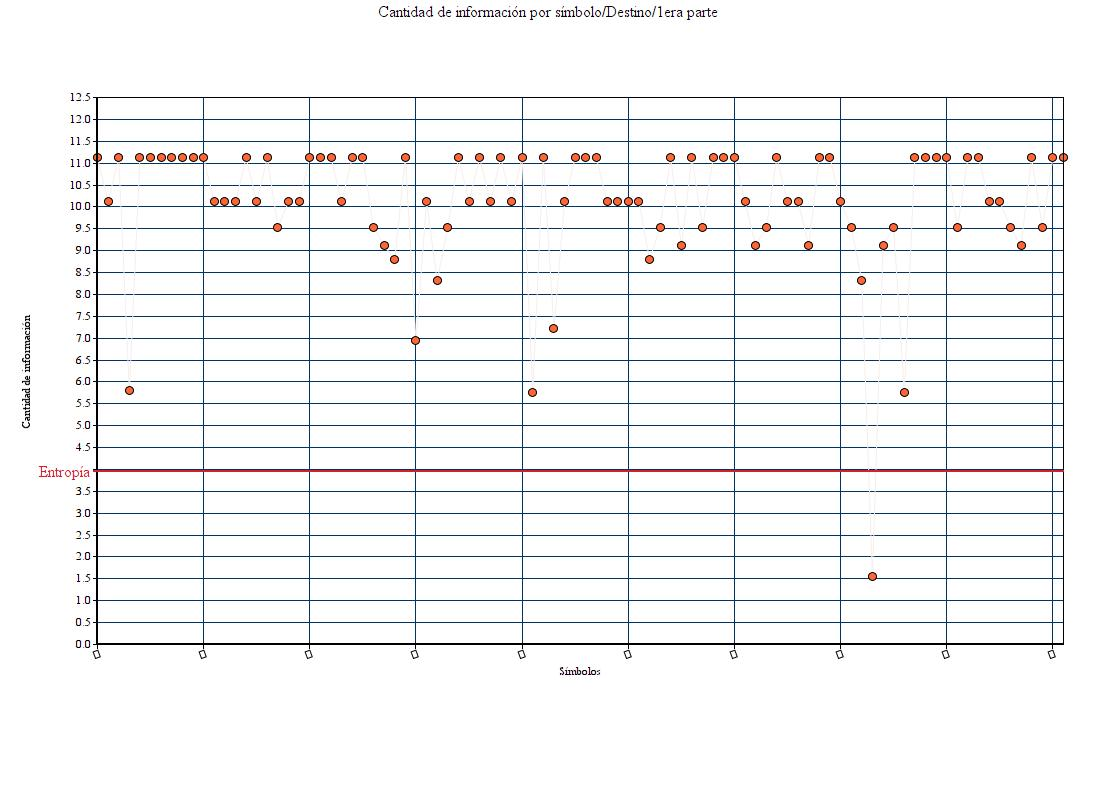
\includegraphics[scale=0.45]{imagenes/graficos/entropiaCantInf/02destino1eraParte.jpg}
  \caption{Cantidad de Información por Símbolo (Destinos) VS Entropía (Parte 1)}
  \label{fig:1}
\end{figure}
\begin{figure}[H]
  \centering
    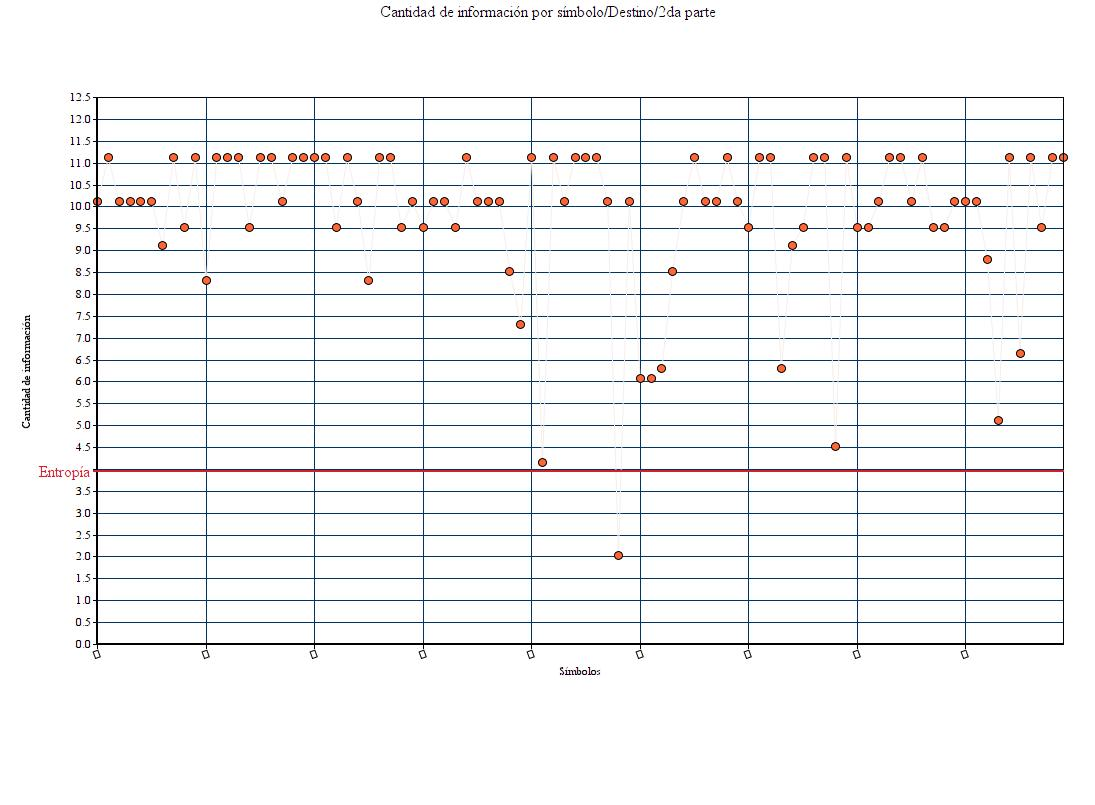
\includegraphics[scale=0.45]{imagenes/graficos/entropiaCantInf/02destino2daParte.jpg}
  \caption{Cantidad de Información por Símbolo (Destinos) VS Entropía (Parte 2)}
  \label{fig:2}
\end{figure}

En las Figuras \ref{fig:1} y \ref{fig:2} , es decir, cuando se tomaron únicamente las direcciones IP de destino en el modelado, se puede ver cómo la mayor parte de los símbolos proveen una gran cantidad de información en contraste con la entropía y también cómo una minoría se destaca por proveer muy poca información. En cambio en las Figuras \ref{fig:3} y \ref{fig:4}, donde se consideraron sólo las direcciones origen, si bien ocurre algo similar a lo anterior, es un poco menos acentuada la diferencia.

\begin{figure}[H]
  \centering
    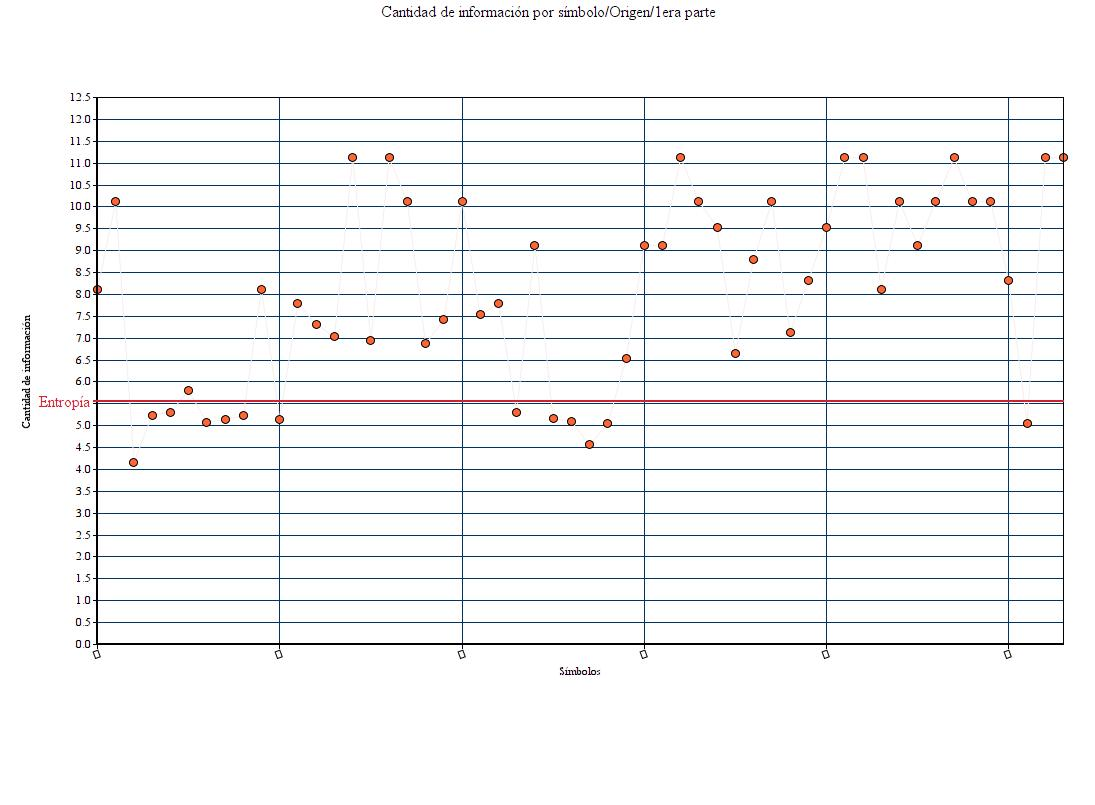
\includegraphics[scale=0.45]{imagenes/graficos/entropiaCantInf/02origen1eraParte.jpg}
  \caption{Cantidad de Información por Símbolo (Orígenes) VS Entropía (Parte 1)}
  \label{fig:3}
\end{figure}


\begin{figure}[H]
  \centering
    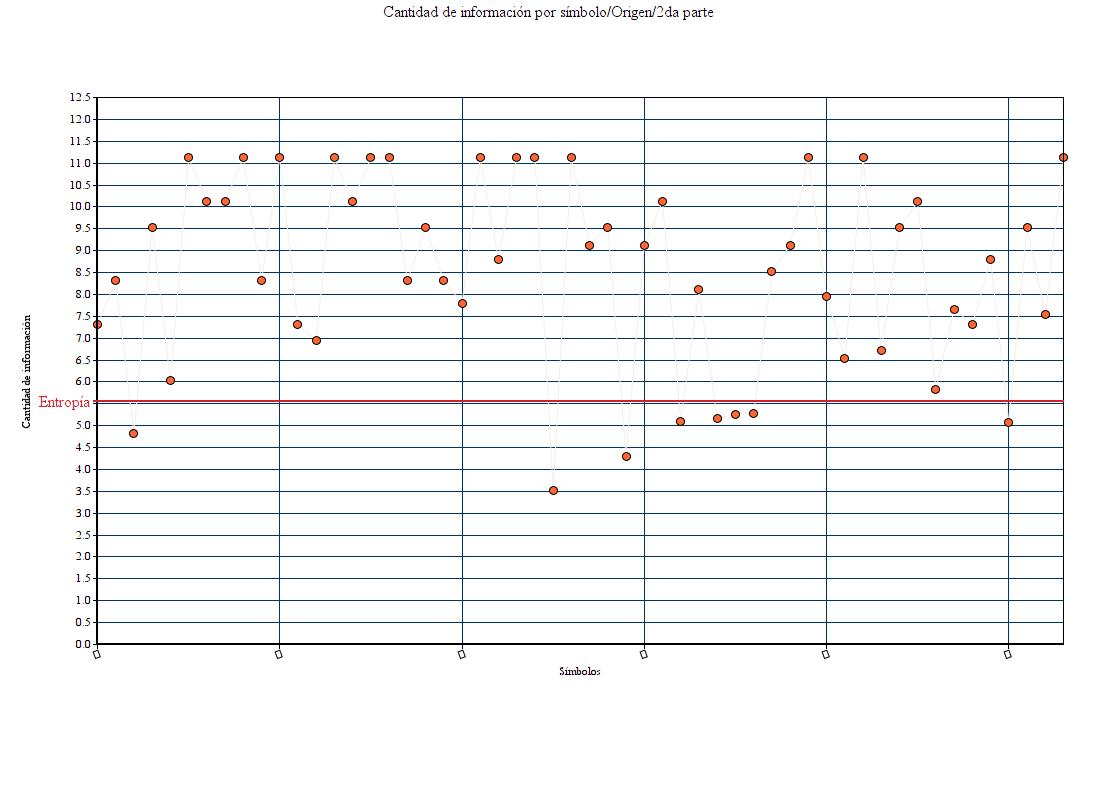
\includegraphics[scale=0.45]{imagenes/graficos/entropiaCantInf/02origen2daParte.jpg}
  \caption{Cantidad de Información por Símbolo (Orígenes) VS Entropía (Parte 2)}
  \label{fig:4}
\end{figure}

\newpage

\begin{figure}[H]
  \centering
    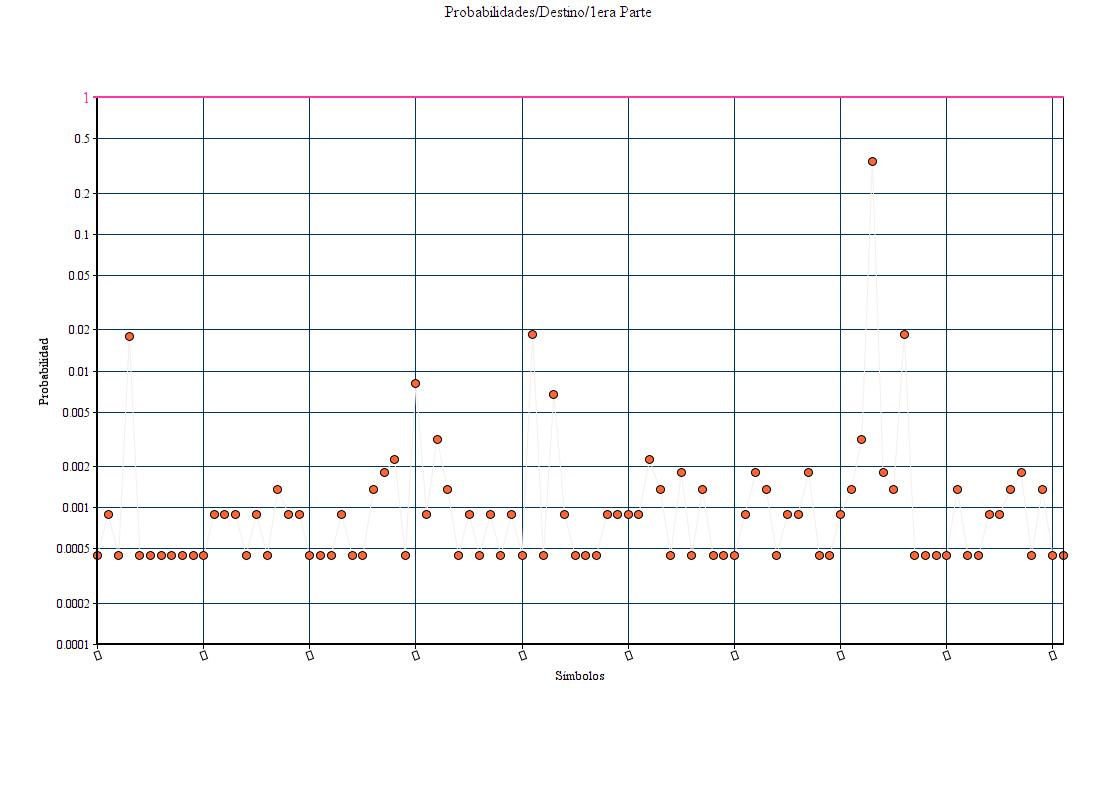
\includegraphics[scale=0.45]{imagenes/graficos/Probabilidades/02destino1eraParte.jpg}
  \caption{Probabilidad de cada Símbolo (Destinos) VS Entropía (Parte 1)}
  \label{fig:5}
\end{figure}

\begin{figure}[H]
  \centering
    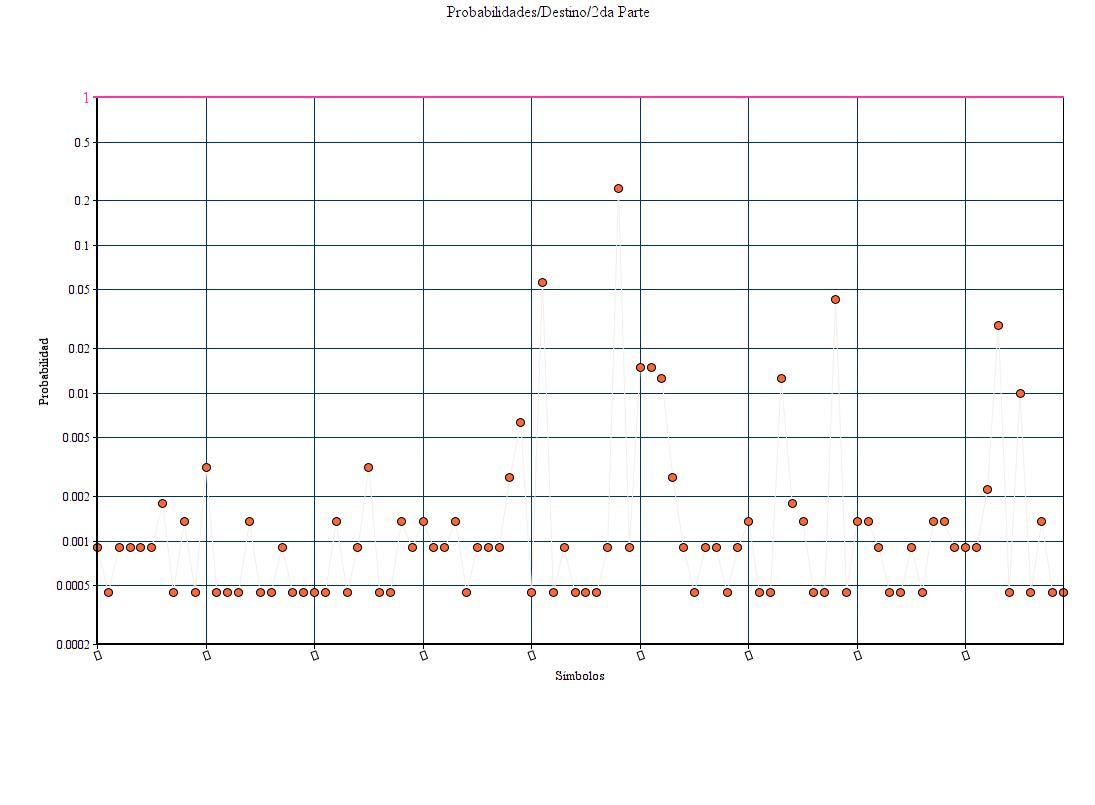
\includegraphics[scale=0.45]{imagenes/graficos/Probabilidades/02destino2daParte.jpg}
  \caption{Probabilidad de cada Símbolo (Destinos) VS Entropía (Parte 2)}
  \label{fig:6}
\end{figure}

\newpage

En el caso de las probabilidades por símbolo ocurre algo análogo a lo que pasaba con la cantidad de información por símbolo, es decir, para los destinos la mayoría tienen una probabilidad muy baja salvo unos pocos que destacan por tener una alta probabilidad, y con los orígenes se presenta algo muy similar pero con las probabilidades un poco más dispersas y no tan marcada la diferencia.

\begin{figure}[H]
  \centering
    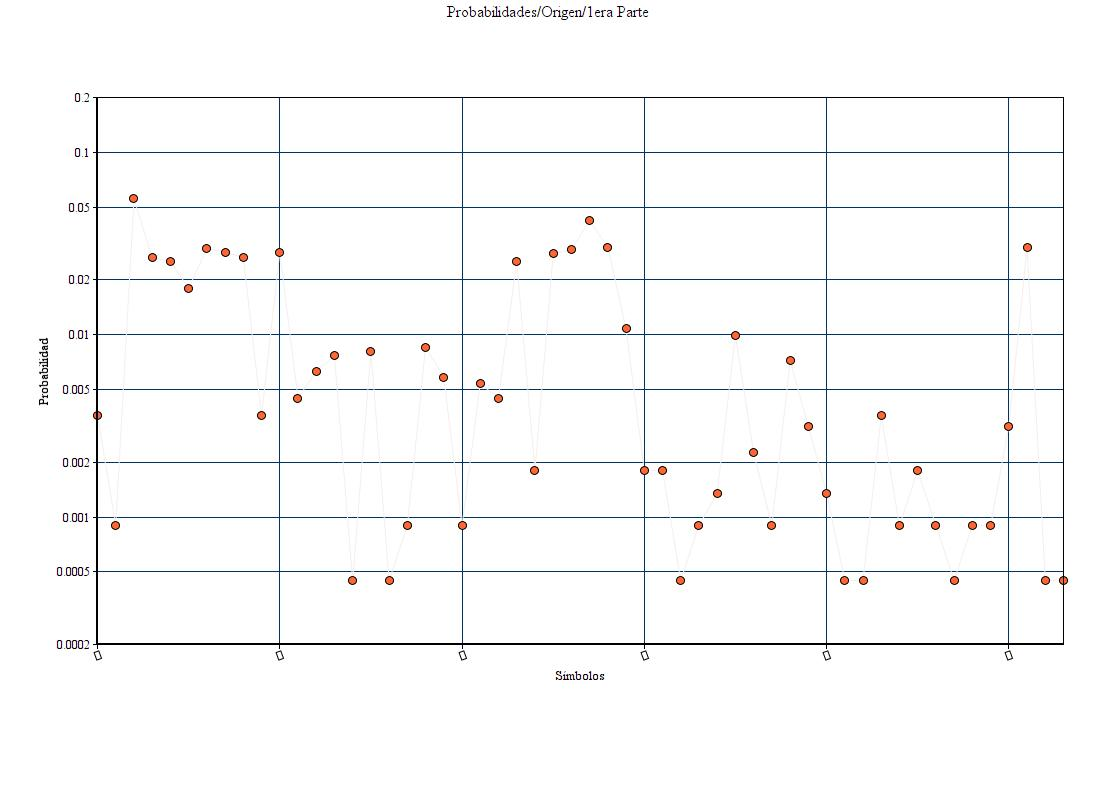
\includegraphics[scale=0.45]{imagenes/graficos/Probabilidades/02origen1eraParte.jpg}
  \caption{Probabilidad de cada Símbolo (Orígenes) VS Entropía (Parte 1)}
  \label{fig:7}
\end{figure}

\begin{figure}[H]
  \centering
    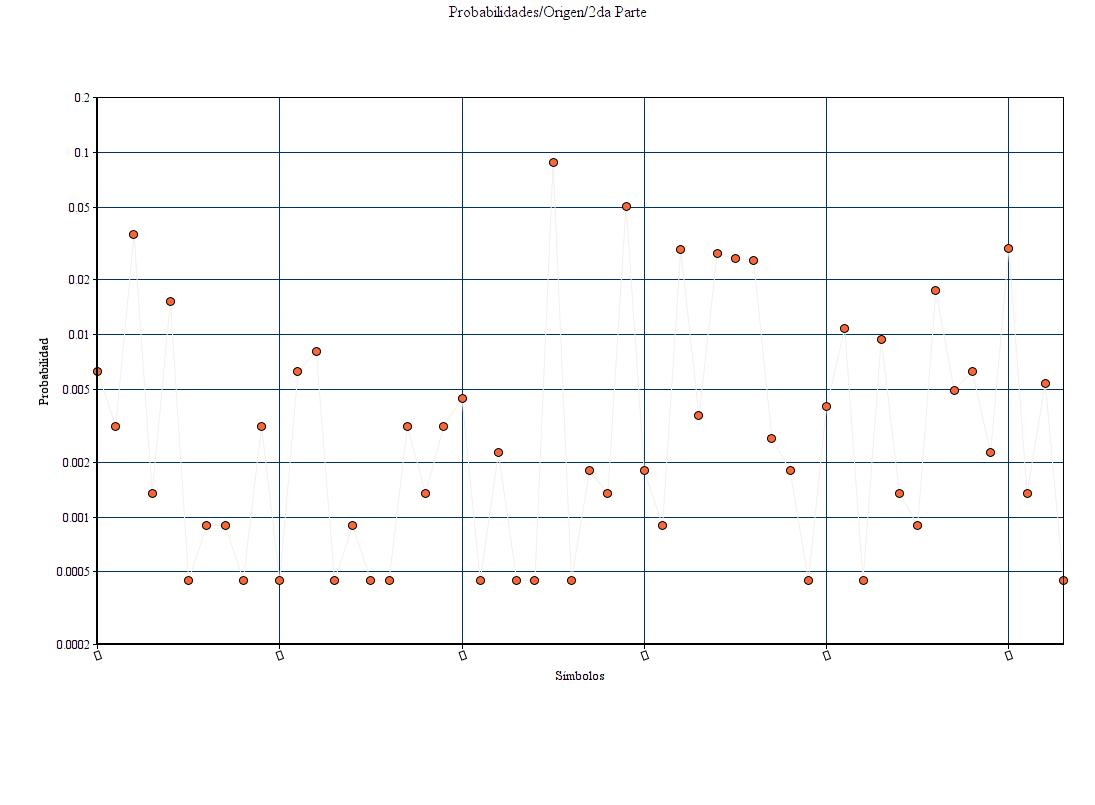
\includegraphics[scale=0.45]{imagenes/graficos/Probabilidades/02origen2daParte.jpg}
  \caption{Probabilidad de cada Símbolo (Orígenes) VS Entropía (Parte 2)}
  \label{fig:8}
\end{figure}

\subsubsection{Experimento 2:}

\begin{figure}[H]
  \centering
    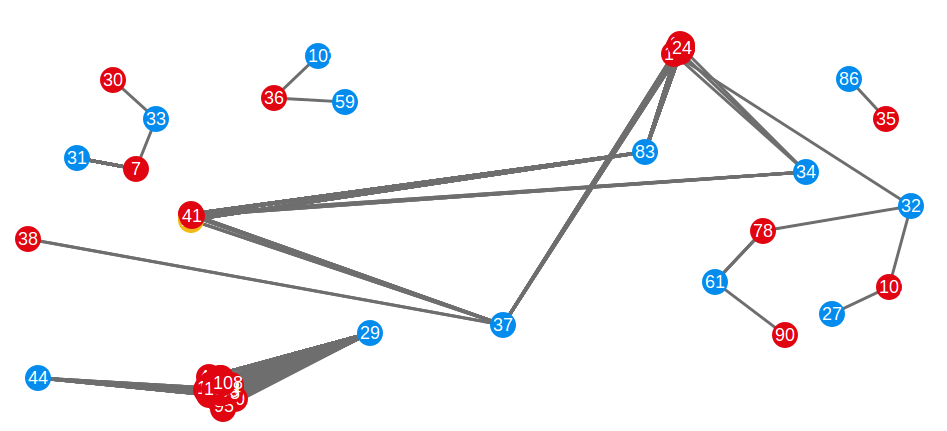
\includegraphics[scale=0.6]{imagenes/graficos/grafos/facultad.png}
  \caption{Red de conexiones entre nodos de la Facultad}
  \label{fig:9}
\end{figure}

En la Figura \ref{fig:9} Se puede observar como el nodo 29 recibe la mayor cantidad de mensajes. También es notoria la red de mensajes formados, entre otros, por el conjunto de nodos liderados por el 24, 41, 37, 83 y 34.

\subsubsection{Experimento 3:}
\begin{verbatim}

Informacion paquetes broadcast: 1.99780228489
Informacion paquetes unicast: 0.415770815585
Entropia: 0.811881635012
Entropia maxima: 1

\end{verbatim}

En estos datos se puede observar una entropía cercana a la entropía máxima.

\newpage
\subsection{Captura de Starbucks}

\subsubsection{Experimento 1:}


\begin{figure}[H]
  \centering
    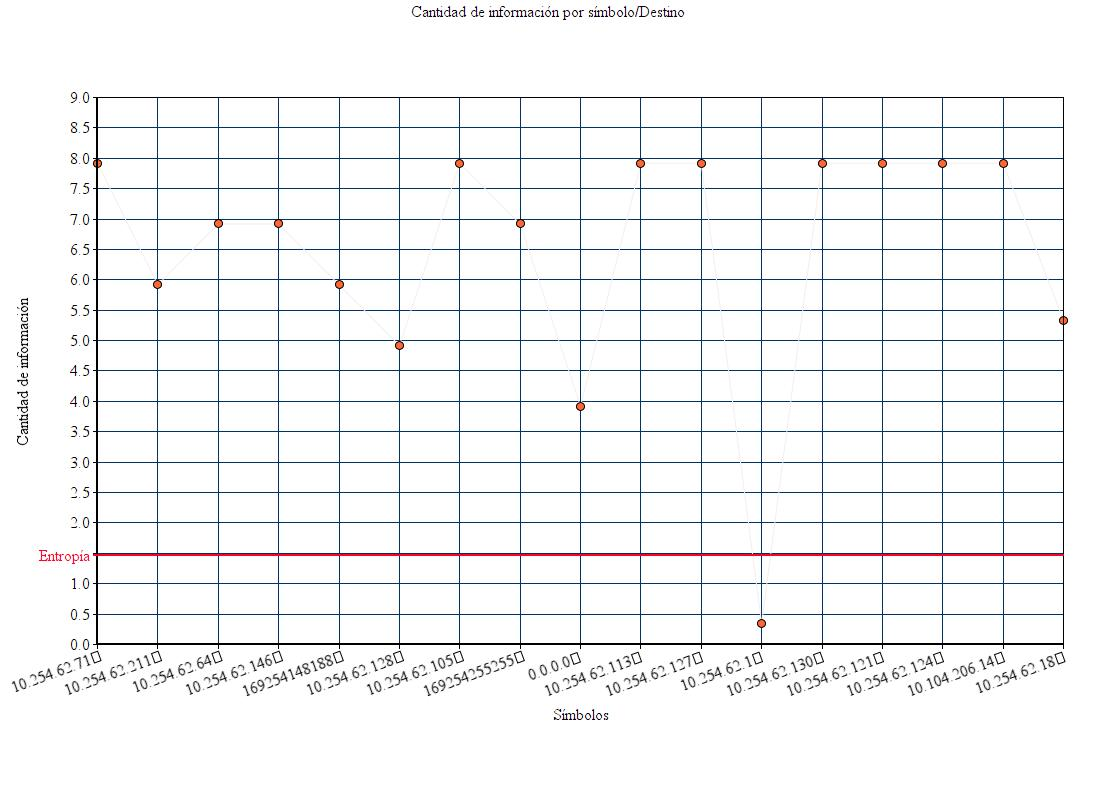
\includegraphics[scale=0.45]{imagenes/graficos/entropiaCantInf/04destino.jpg}
  \caption{Cantidad de Información por Símbolo (Destinos) VS Entropía}
  \label{fig:10}
\end{figure}

\begin{figure}[H]
  \centering
    \includegraphics[scale=0.45]{imagenes/graficos/entropiaCantInf/04origen.jpg}
  \caption{Cantidad de Información por Símbolo (Orígenes) VS Entropía}
  \label{fig:11}
\end{figure}

El resultado observado en las Figuras \ref{fig:10} y \ref{fig:11} es similar al de la red de la Facultad. Es de destacar sin embargo, que la dirección IP 10.254.62.1, aquella que en la Figura \ref{fig:10} muestra la menor cantidad de información, es la dirección del router.

\begin{figure}[H]
  \centering
    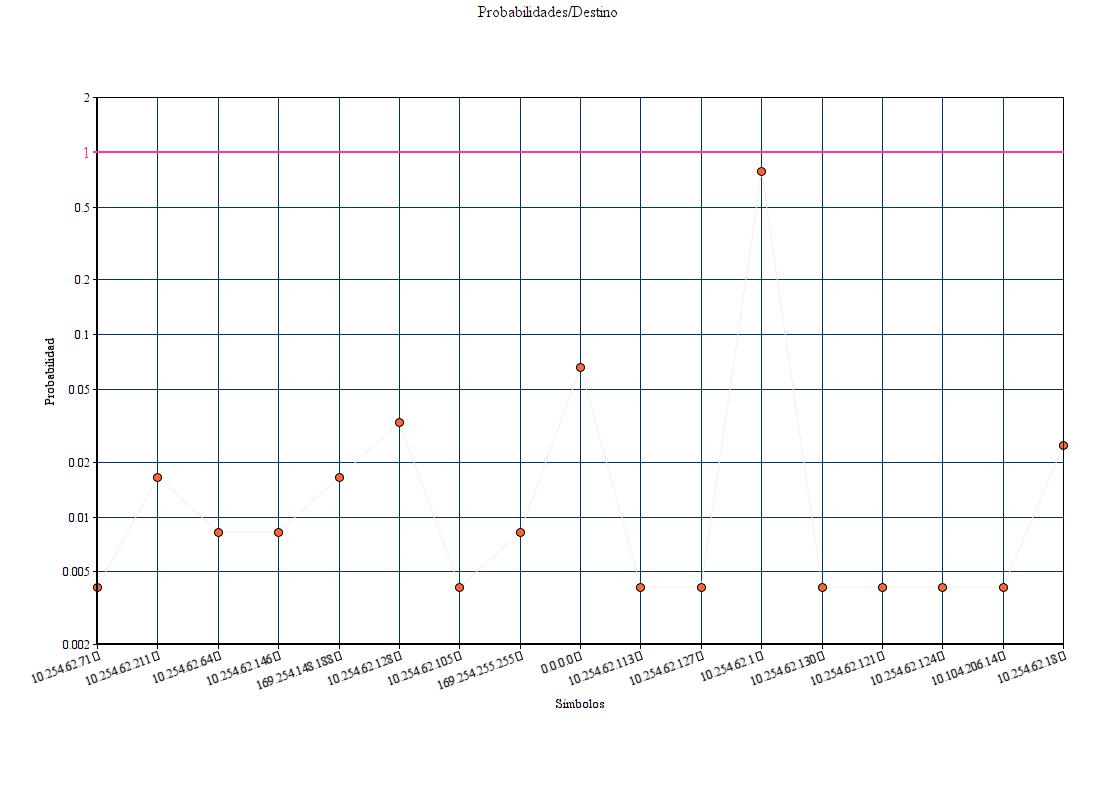
\includegraphics[scale=0.45]{imagenes/graficos/Probabilidades/04destino.jpg}
  \caption{Probabilidad de cada Símbolo (Destinos) VS Entropía}
  \label{fig:12}
\end{figure}

Lo que se observa en los gráficos de probabilidades, Figuras \ref{fig:12} y \ref{fig:13}, no difiere tampoco de lo ocurrido en el caso de las probabilidades de la red de la Facultad.

\begin{figure}[H]
  \centering
    \includegraphics[scale=0.45]{imagenes/graficos/Probabilidades/04origen.jpg}
  \caption{Probabilidad de cada Símbolo (Orígenes) VS Entropía}
  \label{fig:13}
\end{figure}

\subsubsection{Experimento 2:}

\begin{figure}[H]
  \centering
    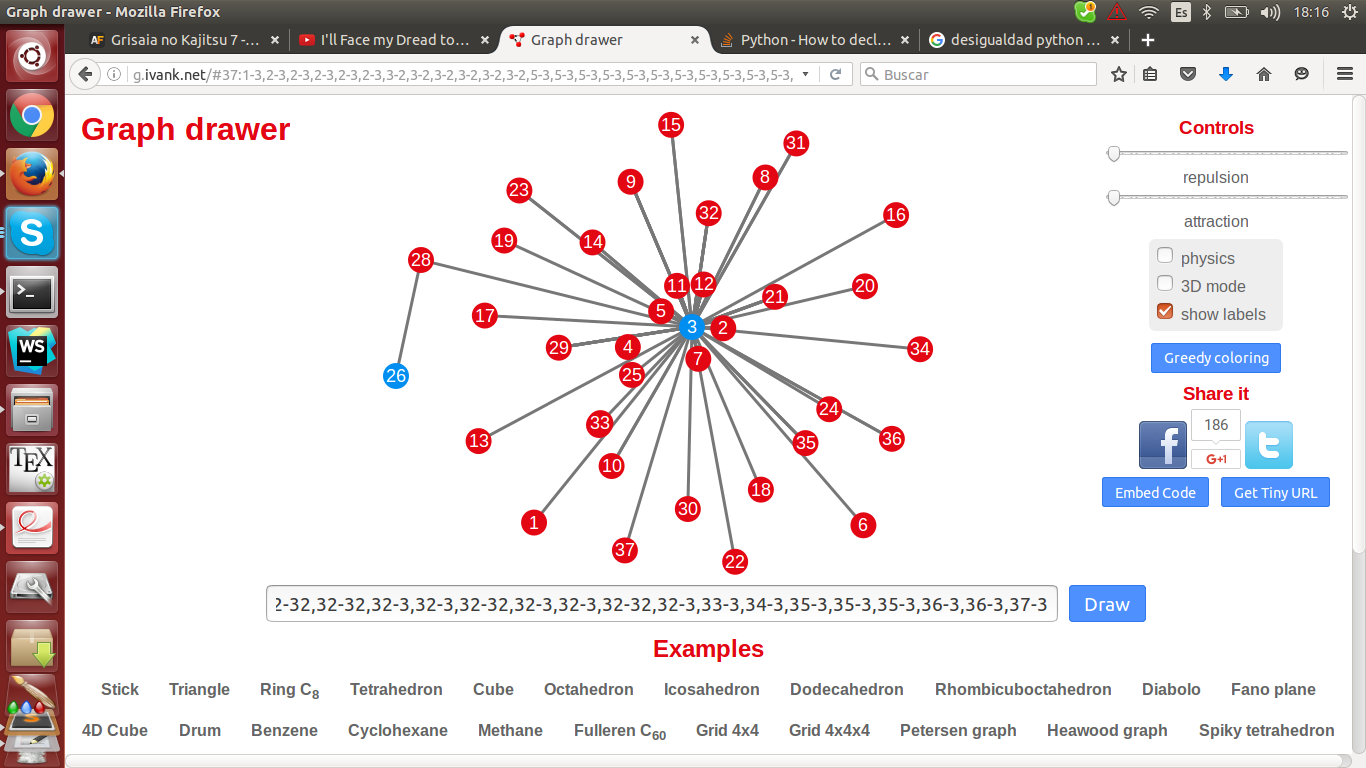
\includegraphics[scale=0.45]{imagenes/graficos/grafos/starbucks.png}
  \caption{Red de conexiones entre nodos de Starbucks}
  \label{fig:14}
\end{figure}

En la Figura \ref{fig:14} se puede observar como todos los nodos tienen conexión con el nodo 3. Es de resaltar, que el nodo 3 representa al router.

\subsubsection{Experimento 3:}
\begin{verbatim}

Informacion paquetes broadcast: 1.92934544644
Informacion paquetes unicast: 0.439379459651
Entropia: 0.830567440737
Entropia maxima: 1

\end{verbatim}

En estos datos se puede observar una entropía cercana a la entropía máxima.

\subsection{Captura del Cyber}

\subsubsection{Experimento 1:}

\begin{figure}[H]
  \centering
    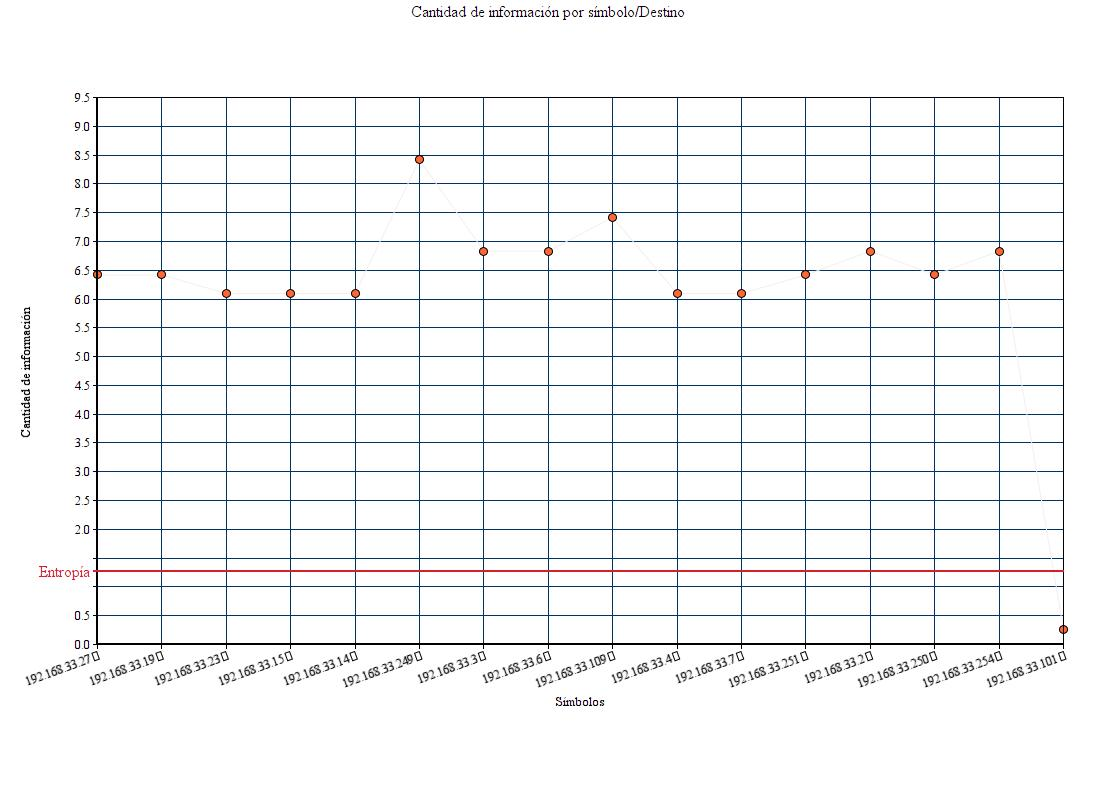
\includegraphics[scale=0.45]{imagenes/graficos/entropiaCantInf/06destino.jpg}
  \caption{Cantidad de Información por Símbolo (Destinos) VS Entropía}
  \label{fig:15}
\end{figure}

El resultado observado en las Figuras \ref{fig:15} y \ref{fig:16} es similar al de las redes de la Facultad y Starbucks pero a una escala mucho menor.

\begin{figure}[H]
  \centering
    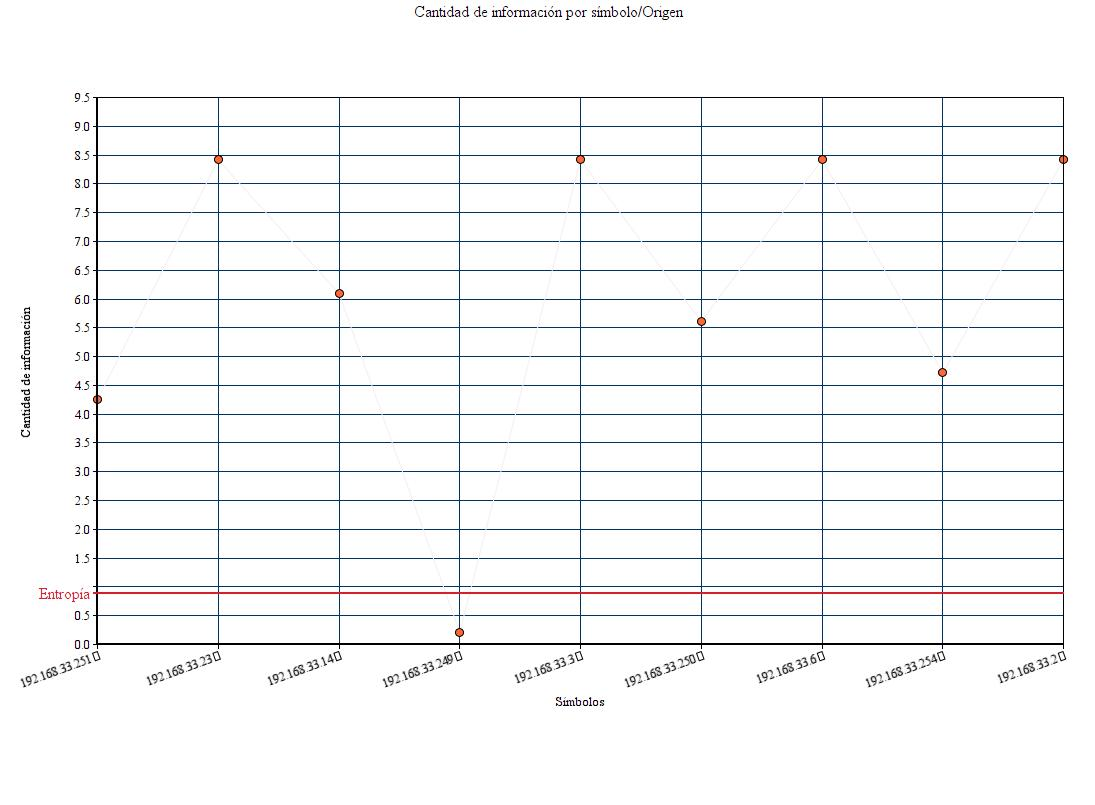
\includegraphics[scale=0.45]{imagenes/graficos/entropiaCantInf/06Origen.jpg}
  \caption{Cantidad de Información por Símbolo (Orígenes) VS Entropía}
  \label{fig:16}
\end{figure}

\begin{figure}[H]
  \centering
    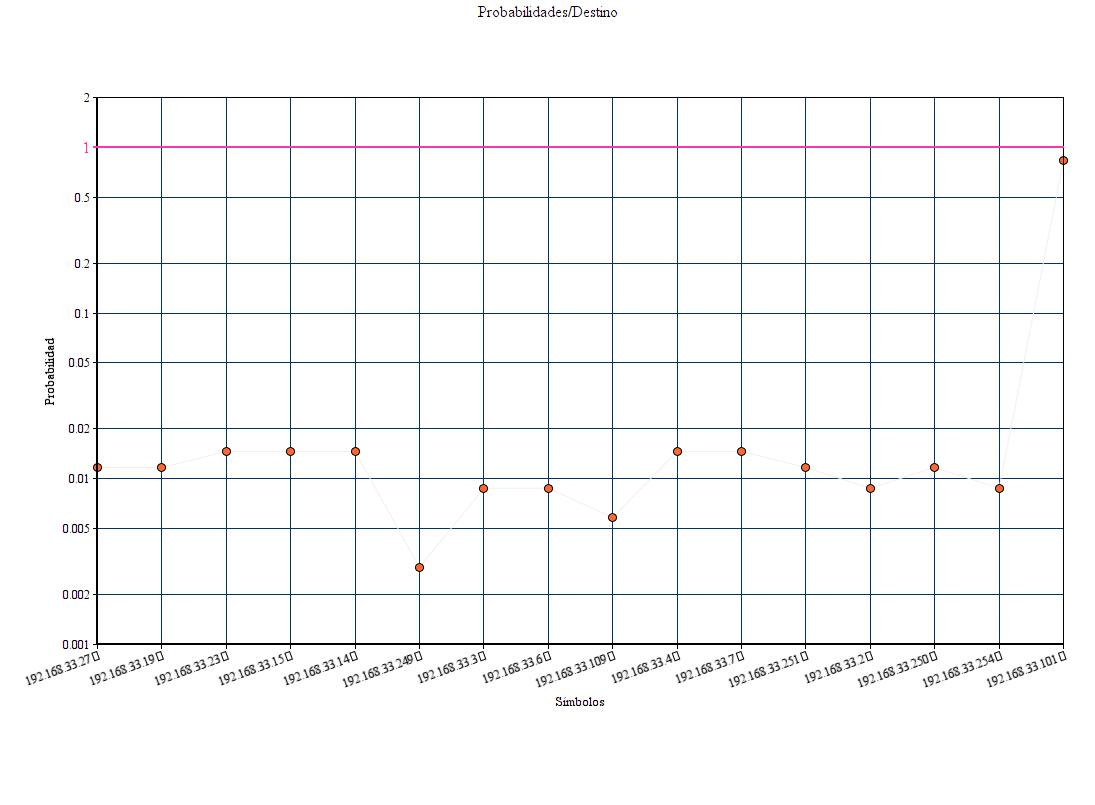
\includegraphics[scale=0.45]{imagenes/graficos/Probabilidades/06destino.jpg}
  \caption{Probabilidad de cada Símbolo (Destinos) VS Entropía}
  \label{fig:17}
\end{figure}

Como se puede ver en las Figuras \ref{fig:17} y \ref{fig:18}, las probabilidades no se salen del patrón que se repite tanto en la red de la Facultad como en la de Starbucks.

\begin{figure}[H]
  \centering
    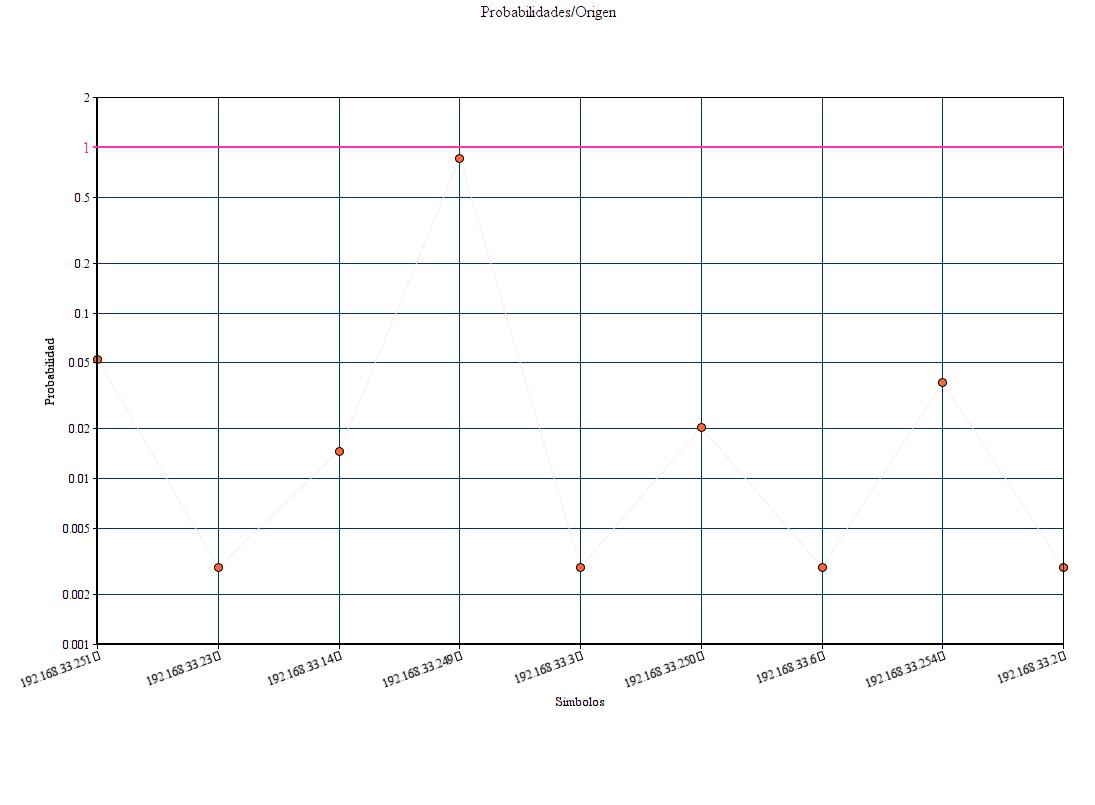
\includegraphics[scale=0.45]{imagenes/graficos/Probabilidades/06origen.jpg}
  \caption{Probabilidad de cada Símbolo (Orígenes) VS Entropía }
  \label{fig:18}
\end{figure}

\subsubsection{Experimento 2:}

\begin{figure}[H]
  \centering
    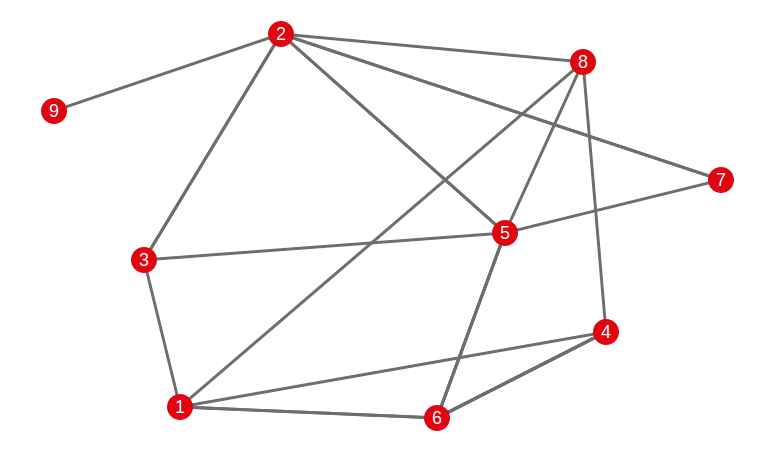
\includegraphics[scale=0.75]{imagenes/graficos/grafos/cyber.png}
  \caption{Red de conexiones entre nodos del Cyber}
  \label{fig:19}
\end{figure}

En el grafo de la Figura \ref{fig:19} se puede apreciar que la mayor concentración de enlaces reside en los nodos 11, 1 y 3, con 12, 10 y 8 vecinos cada uno respectivamente, en contraposición con el resto, que tienen a lo sumo 5 vecinos cada uno.

\subsubsection{Experimento 3:}

\begin{verbatim}

Informacion paquetes broadcast: 4.45787627635
Informacion paquetes unicast: 0.0671883016179
Entropia: 0.266980303664
Entropia maxima: 1

\end{verbatim}

En estos datos se puede observar una entropía lejana a la entropía máxima.